\documentclass{article}
\usepackage{amsmath}
\usepackage[utf8]{inputenc}
\usepackage{hyperref}
\hypersetup{
    colorlinks=true,
    linkcolor=blue,
    filecolor=magenta,
    urlcolor=blue,
}
\usepackage{graphicx}

\usepackage{fullpage}
\newcommand{\amy}[1]{{\color{blue}[Amy: #1]}}
\newcommand{\jason}[1]{{\color{red}[Jason: #1]}}
\newcommand{\eli}[1]{[Eli: #1]}

\title{CSCI1410 Fall 2020 \\
Assignment 2: Adversarial Search}

\date{Code Due Monday, October 12 at 11:59 ET \\ [1ex]
Writeup Due Tuesday, October 13 at 11:59 ET}

\begin{document}

\maketitle


\section{Goals}
In this assignment, you will implement two adversarial search algorithms,
minimax and alpha-beta pruning.
You will also develop an evaluation function for Tic-Tac-Toe.
You will use the aforementioned machinery to solve multiple instances of Tic-Tac-Toe and Connect Four,
reporting on the success of your implementations and evaluation function on games of increasing complexity.


\section{Introduction}
Perhaps all of you have played \href{https://en.wikipedia.org/wiki/Tic-tac-toe}{Tic-Tac-Toe},
also known as Noughts and Crosses.
If not, you can try it out \href{https://playtictactoe.org/}{here}.
Even if so, you may not have played on a 4$\times$4 or a 5$\times$5 board before.
In this assignment, you will have a chance to play against an adversarial search algorithm on boards of various sizes.

\href{https://en.wikipedia.org/wiki/Connect_Four}{Connect Four} is another popular children's game.%
\footnote{Actually, it is also popular with dogs: \url{https://www.youtube.com/watch?v=kFvBtSpZ3DY}.}
Connect Four is a solved game, from the start state.
In particular, a winning strategy for the first player is known.
A losing strategy for the first player is also known.
This game was solved by man, not machine,
but machines later verified manually derived solutions
using enhanced versions of minimax search and alpha-beta pruning.

These two games form the basis of this assignment,
but the algorithms you will implement to solve these games apply to all
deterministic, two-player, zero-sum games of perfect information.


\section{Data Structures}
We have implemented Tic-Tac-Toe and Connect Four for you.
We did so as an instantiation of an abstract class called
\verb|AdversarialSearchProblem|---defined in \verb|adversarialsearchproblem.py|---which
includes fields for all the usual components of two-player games:
what the start and end states are,
whose turn it is,
what actions are available at each state,
where the game state transitions to from a state given an action,
and a function that evaluates states.
%As always, when coding, the first step is to fully comprehend your data.
%As such,
We recommend that you fully comprehend
\verb|AdversarialSearchProblem| before you attempt to
implement any search algorithms that operate on this data structure.


\section{Algorithms}
Once again, the algorithms you will implement in this assignment are minimax and alpha-beta pruning.
As you scale up, however, to bigger and bigger versions of games (e.g., Tic-Tac-Toe on 4$\times$4 or
5$\times$5 boards),
you will find that these algorithms cannot complete the search in a reasonable amount of time.
As a result, you will also implement alpha-beta pruning to a fixed depth (also called a \textit{ply}).
But note that doing so requires that you define (and implement) a function
capable of evaluating \emph{all\/} intermediate game states.

We have implemented a sample evaluation function for you, within the Connect Four game implementation.
Here is how it works:
Define a \textbf{slice} on a Connect Four board as
four connected slots that would result in a win if occupied by one player.
Now, the evaluation function totals up the score of all slices at the current state,
for the current player, where each slice is scored as follows:
\begin{itemize}
  \item 100 points if all 4 slots are occupied by the given player,
  \item 5 points if 3 slots are occupied by the given player and 1 is empty,
  \item 2 points if 2 slots are occupied by the given player and 2 are empty,
  \item $-$4 if 3 slots are occupied by the opponent and 1 is occupied by the given player, and
  \item 0 points otherwise.
\end{itemize}
As you can see, evaluation functions are heuristics that are developed using domain knowledge.
%The example evaluation function runs with a cutoff of 4 by default, but feel free to experiment with this value!


\section{Your Task}
Your primary task in this assignment is to implement several adversarial search algorithms.
After implementing these algorithms, you will run a series of experiments to test them on games of varying size,
and you will summarize your findings.
You might find, for example, that minimax can only solve Tic-Tac-Toe on boards of size 3,
but that it fails on boards of size 4.
In contrast, alpha-beta pruning may solve Tic-Tac-Toe on boards of size 4,
but it may not solve Connect Four.
For small enough plies, limited-ply alpha-beta pruning always returns a solution;
those solutions, however, need not resemble winning strategies.


\subsection{Coding}
In \verb|adversarialsearch.py|, you will implement the following three functions,
each of which takes in an \verb|AdversarialSearchProblem| and outputs an action for the player whose turn it is.

\begin{enumerate}
\item \verb|minimax|. Implement the minimax algorithm for two-player, zero-sum games.
  Your implementation should search all the way down to terminal states.

  Once you think you have a working implementation of \verb|minimax|, try it out on Tic-Tac-Toe.
  To do so, run \verb|python gamerunner.py| from the command line.
  By default, the \verb|run_game| function in \verb|python gamerunner.py|
  sets up a game of Tic-Tac-Toe between a minimax agent and you!
  (Be sure to activate the virtual environment first!)

\item \verb|alpha_beta|. Implement alpha-beta pruning.

  After implementing \verb|alpha_beta|,
  play Tic-Tac-Toe against your new implementation by invoking \verb|run_game| as follows:
  \verb|python gamerunner.py --player2=ab|.

  Notice any speed difference?

  Now, try playing Connect Four:
  \verb|python gamerunner.py --player2=ab --game=connect4|

  You may try waiting a little while, but the program will not terminate any time soon, unless you intervene
  (type \verb|CTRL-C| in console).

\item \verb|alpha_beta_cutoff|. Implement alpha-beta pruning to a fixed ply, at which point an
  evaluation function is applied.

  With a cutoff, alpha-beta pruning can make faster decisions, but are they any good?
  Try it out on Connect Four by choosing a cutoff, say 4, and running:

  \verb|python gamerunner.py --player2=ab-cutoff --cutoff=4 --game=connect4|
\end{enumerate}

You may assume that game is \textbf{alternating move}. This means that the second player always
takes his turn after the first player, and the first player always takes her turn after the second
player. \textbf{You should not assume that you are the first player to move, and you should aim
to maximize your score.}

Finally, using your knowledge of the game, write an evaluation
function for Tic-Tac-Toe, meaning a function that ascribes a score to
all possible Tic-Tac-Toe board configurations.  A stub for this
function, \verb|eval_func|, can be found in \verb|tttproblem.py| (and needs to be defined in every ASP implementation running \verb|alpha_beta_cutoff|, for that matter).
%
For your reference,
our evaluation function for Connect Four \verb|eval_func| is included in \verb|connect4problem.py|.


\subsection{Written Questions}
In addition to your code, you should also submit a PDF file in which you
answer the following questions, one at a time.  While not required, we
recommend that you use \LaTeX{} to typeset your work.

\begin{enumerate}
  \item Describe your evaluation function. Explain why it is sensible.

  \item Design and run experiments to test the various algorithms on Tic-Tac-Toe games of varying size.
    Test minimax and alpha-beta pruning on smaller games,
    and alpha-beta pruning with a variable cutoff on bigger games.
    Report your findings in a table, and summarize them in a few sentences.

    Your table/summary should answer questions like:
    How often do minimax and alpha-beta pruning succeed,
    as a function of the size of the game?
    How well does alpha-beta pruning with a cutoff play, as a function of the cutoff?
    And how does its accuracy vary with its run time?
\end{enumerate}

\if 0
A friend says, ``Use the minimax algorithm if you can!
It produces the best decisions possible in two-player, zero-sum games.''
Do you agree with this assertion?
If not, give at least two reasons why you think the assertion is wrong.
Only consider situations where minimax is actually feasible to use.
Limit your response to 3 sentences.
\fi


\subsection{Ethics Questions}
Like all games, video games are games in the game-theoretic sense. Read \href{https://www.gamasutra.com/blogs/CeliaHodent/20191220/356013/Ethics_in_the_Videogame_Industry_A_Mythbusting_and_Scientific_Approach.php}{this article} about ethics in the video game industry, paying particular attention to Sections 2 and 3, and then answer the following questions.

\begin{enumerate}
  \item Hodent argues that loot boxes should be regulated. Do you find her rationale convincing? If not, why not? If so, which regulations among those she suggests would you expect to be the most viable, and related, the most effective?

  \item Hodent states that it is ``not always clear if a design is a dark pattern or not: it depends on the context and mostly on the intention behind.'' Describe an interaction with a video game, an app, or other technology service that you feel constitutes a dark pattern? (Feel free to attach a screenshot if it would enhance your explanation.) Is there an alternative context in which the dark pattern you describe could have positive implications?
\end{enumerate}


\noindent
Please submit your writeup via Gradescope (see the Gradescope guide on the course website for more details).

\section{The Code Files}
\subsection{Files to Modify}
\begin{itemize}
  \item \verb|adversarialsearch.py| - This is where you will code the adversarial search algorithms.

  \item \verb|tttproblem.py| - This is where you will code your evaluation function for Tic-Tac-Toe (and where the rest of the game is implemented).
\end{itemize}


\subsection{Core Source Code}
\begin{itemize}
  \item \verb|adversarialsearchproblem.py| contains two abstract classes relevant to search algorithms: \\
    \verb|AdversarialSearchProblem| and \verb|GameState|.

%    \verb|AdversarialSearchProblem| is analogous to \verb|SearchProblem| from the previous assignment; it contains methods that all adversarial search problems have in common.
    All of the algorithms that you will implement in this assignment take in an \verb|AdversarialSearchProblem|.

    The \verb|GameState| class is also abstract.
    It represents a game state.
    The only requirement that is imposed by the \verb|GameState| class is that a game state implement the \verb|player_to_move| method, which returns the player whose turn it is.
\end{itemize}


\subsection{Testing Source Code}
\begin{itemize}
  \item \verb|gamedag.py| implements an \verb|AdversarialSearchProblem| as a game DAG (directed, acyclic graph).
    You can use the \verb|GameDAG| class to create simple, abstract adversarial search problems for testing purposes.
    Read the \verb|GameDAG| class's docstrings to learn how to create a \verb|GameDAG|.

  \item \verb|unit_tests.py| includes basic test cases and correctness checks for simple game trees.
    Below you can see a visualization of the game tree created in the \verb|_get_test_dag| function in \verb|unit_tests.py|.
    You can test your various implementations by running them on the game trees generated by
    \verb|_get_test_dag| and \verb|_get_test_dag_2|.
    These tests should should take no more than 1 second.
\end{itemize}

%\begin{figure}[ht!]
\centerline{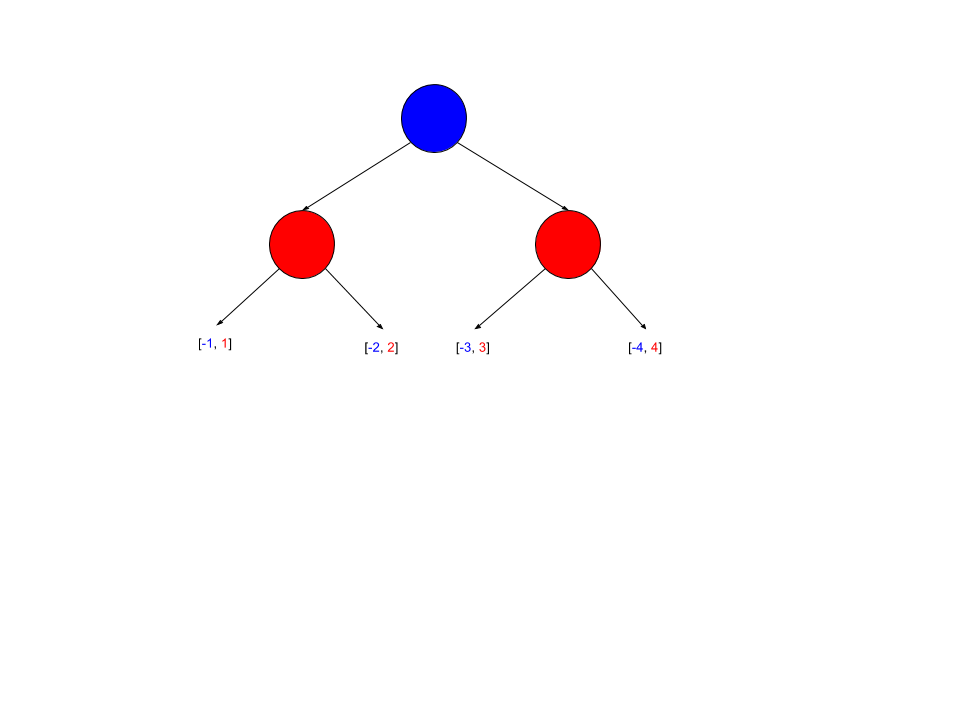
\includegraphics[scale = 0.33]{example-DAG.png}}
%\label{fig:test}
%\end{figure}


\mbox{}
\vspace{-1.75in}

\subsection{Game Runner}\label{gamerunner}
We have implemented Tic-Tac-Toe and Connect Four as instances of \verb|AdversarialSearchProblem| for you,
so that you can play these games, and see the algorithms come to life!
%To play, you type \verb|python gamerunner.py| at the command line.

\begin{itemize}
\item You can find our implementations of Tic-Tac-Toe and Connect Four in
  \verb|asps/tttproblem.py| and \verb|asps/connect4problem.py|, respectively.
  Both are equipped with \verb|GameUI|s (User Interface), written for visualization via
  \verb|gamerunner.py|.

%\verb|asps/connect4problem.py| also contains an example evaluation function belonging to the \verb|Connect4Problem| class called \verb|eval_func|, which you can use as a reference when designing your evaluation function for \verb|TTTProblem|.

\item The main function in \verb|gamerunner.py| runs an instance of Tic-Tac-Toe,
  where the players are by default you and a minimax agent.
  This default behavior is equivalent to running:

  \verb|python gamerunner.py --player1=self --player2=minimax --game=ttt|

  To play Connect Four instead of Tic-Tac-Toe, use \verb|--game=connect4|.

  To play against different agents, or to see how different algorithms
  play against each other, change the players to \verb|self|,
  \verb|minimax|, \verb|ab|, or \verb|ab-cutoff|.

  When choosing \verb|ab-cutoff| to be a player, you must provide a
  ply, or depth at which to cut off the search and call the evaluation
  function to estimate state values.  To set this value, use the
  \verb|--cutoff| argument. For example:

  \verb|python gamerunner.py --player2=ab-cutoff --cutoff=5|

  If you want to vary the size of the board for either game, you can
  do so by passing in the optional argument \verb|--dimension=dim|,
  which constructs a \verb|dim|$\times$\verb|dim| board. (Note
  that \verb|dim| must be at least 3 for Tic-Tac-Toe and at least 4
  for Connect Four.) Here is an example:

  \verb|python gamerunner.py --game=connect4 --dimension=5|

  To see a summary of all of available options, from the command line, simply run:

  \verb|python gamerunner.py --help|
\end{itemize}

\noindent
Our \verb|gamerunner.py| implementation works for any \verb|AdversarialSearchProblem|,
so if you create a new game, you can play it using \verb|python gamerunner.py --game=custom| (take a look at the file for instructions on including your own ASP, if you want).


\section{Help}
You can find pseudocode for the minimax algorithm on page 166 of the textbook.
You can find pseudocode for the alpha-beta pruning algorithm on page 170 of the textbook.
Note that you will need to modify the pseudocode to work with \verb|AdversarialSearchProblem|s.


\section{Grading}
We will give you your score based on the rubric in \verb|rubric.txt|.
Here are some details about the rubric:

\begin{itemize}
  \item For both \verb|alpha_beta| and \verb|alpha_beta_cutoff|, you will earn points if your implementation ``expands game states in a correct way,'' meaning that it visits only the game states it should.
  To evaluate this, the autograder will look only at the sequence of (\verb|GameState|, \verb|action|) pairs on which \verb|transition(.)| is called.
  What we're looking for here is that, in whatever order your implementation's visit the game states, they prune all the branches that they should when visiting in that order.
  To test this, you can create a \verb|GameDAG| and check that your implementations do not visit states that should be pruned.

  \item Finally, please avoid superfluous calls to \verb|transition(.)|, as they will throw off the autograder.
\end{itemize}


\section{Install and Handin Instructions}
To install, run \verb|cs1410_install Adversarial_Search| in \verb|~/course/cs1410|.

To hand in, run \verb|cs1410_handin Adversarial_Search| in
\verb|~/course/cs1410/Adversarial_Search|,
which should contain your \verb|adversarialsearch.py|.

In addition, please submit the written portion of the assignment via Gradescope.

In accordance with the course \href{https://forms.gle/DqfbBY8jdaqenRoa9}{grading policy}, your
written homework should not contain your name, Banner~ID, CS~login, or any other personally
identifiable information.

\end{document}
